
\documentclass[12pt, a4paper]{article}

%-----------USEPACKAGE----------------------------
\usepackage{bm} % Tucne pismo
\usepackage[czech]{babel} % Cestina
\usepackage[T1]{fontenc}
\usepackage[utf8x]{inputenc}
\linespread{1.10} % Radkovani 1.3 odpovida radkovani 2
\usepackage{lmodern} % Daji se pouzit \HUGE atd.
\usepackage{amsmath}
\usepackage{algorithm}
\usepackage[noend]{algpseudocode} % Vkladani pseudo kodu
\usepackage{listings}
\usepackage{setspace}

% Graphics
\usepackage{graphicx}
\usepackage{epstopdf}
\usepackage{color}
\graphicspath{{./img/}}

% Hyperref and its color
\usepackage[unicode]{hyperref} % Odkazy v pdf, www a na e-mail
\usepackage[hypcap=true]{caption}
\usepackage[hypcap=true,list=true]{subcaption}
\hypersetup{colorlinks = true, citecolor = black}
\hypersetup{linkcolor=red}
\hypersetup{colorlinks,urlcolor=black}

%-----------COLORS--------------------------------
\definecolor{Code}{rgb}{0,0,0}
\definecolor{Decorators}{rgb}{0.5,0.5,0.5}
\definecolor{Numbers}{rgb}{0.5,0,0}
\definecolor{MatchingBrackets}{rgb}{0.25,0.5,0.5}
\definecolor{Keywords}{rgb}{0,0,1}
\definecolor{self}{rgb}{0,0,0}
\definecolor{Strings}{rgb}{0,0.63,0}
\definecolor{Comments}{rgb}{0,0.63,1}
\definecolor{Backquotes}{rgb}{0,0,0}
\definecolor{Classname}{rgb}{0,0,0}
\definecolor{FunctionName}{rgb}{0,0,0}
\definecolor{Operators}{rgb}{0,0,0}
\definecolor{Background}{rgb}{1, 1, 1}

%-----------LISTINGS-SETTINGS----------------------
\lstset{
	numbers=left,
	numberstyle=\footnotesize,
	numbersep=0.5em,
	xleftmargin=1.5em,
	xrightmargin=0em,
	framextopmargin=0em,
	framexbottommargin=0em,
	showspaces=false,
	showtabs=false,
	showstringspaces=false,
	frame=lrtb,
	tabsize=4,
	% Basic
	basicstyle=\ttfamily\footnotesize\setstretch{1},
	backgroundcolor=\color{Background},
	language=Python,
	% Comments
	commentstyle=\color{Comments}\slshape,
	% Strings
	stringstyle=\color{Strings},
	morecomment=[s][\color{Strings}]{"""}{"""},
	morecomment=[s][\color{Strings}]{'''}{'''},
	% Keywords
morekeywords={import,from,class,def,for,while,if,is,in,elif,else,not,and,or,print,break,continue,return,True,False,None,access,as,del,except,exec,finally,global,import,lambda,pass,print,raise,try,assert},
	keywordstyle={\color{Keywords}\bfseries},
	% Additional keywords
	morekeywords={[2]@invariant},
	keywordstyle={[2]\color{Decorators}\slshape},
	emph={self},
	emphstyle={\color{self}\slshape},
	breaklines=true, % Zalamuje radky.
}







%------------------VARIABLES----------------------------
\newcommand{\cisloCviceni}{1. cvičení}









%------------------LAYOUT----------------------------
\usepackage[top = 2.5 cm, bottom = 2.5 cm, left = 2.5 cm, right = 2.5 cm]{geometry} % geometrie stranky
\usepackage{longtable}% Pro dlouhy obsah, da se zalomit \pagebrek
\usepackage{fancyhdr}
\pagestyle{fancy}% Deffaultni nastaveni hlavicky a paticky
\setlength{\headheight}{16 pt}% Zvetsi hlavicku, aby to nedelalo warningy
\fancyhf{}
\lhead{\href{http://www.kky.zcu.cz/cs/courses/mpv}{Metody Počítačového Vidění}}
\rhead{\cisloCviceni}
\fancyfoot[R]{\thepage}
\fancyfoot[L]{Verze 2.0.0, poslední úpravy: \today}








%---------------BEGIN-DOCUMENT--------------------------
\begin{document}
 









 
%--------TITLE-PAGE--------------------------------------------
\begin{titlepage}
\begin{center}
	
\includegraphics[trim = 0.6cm 0.5cm 0.9cm 0.5cm, scale=1]{FAV_logo_cz.pdf}
	\hspace*{\fill}
	
\includegraphics[trim = 3.5cm 1.5cm 2.6cm 2cm, scale=0.295]{./KKY_logo_cz.pdf}\\
	\vspace*{\fill}
	\textbf{\Huge{\href{http://www.kky.zcu.cz/cs/courses/mpv}{Metody Počítačového Vidění} \\ ~ \\ \cisloCviceni}}\\
	\vspace*{\fill}
	\textbf{\large{\href{mailto:LBures@kky.zcu.cz}{Ing. Lukáš Bureš}}} \hfill \textbf{\large{Plzeň, \today}}
\end{center}
\end{titlepage}












%--------OBSAH-CVICENI---------------------------------
\section*{Obsah cvičení}
\begin{enumerate}
	\item Podmínky získání zápočtu a obecné informace.
	\item Systém automatické kontroly semestrálních prací
	\item Stručné informace o \href{https://www.python.org/}{Pythonu} a \href{http://opencv.org/}{OpenCV (Open Source Computer Vision)}.
	\item Praktické cvičení část 1.: Načítání a konverze obrázku, výpočet histogramu a distribuční funkce, globální ekvalizace histogramu, Contrast Limited Adaptive Histogram Equalization (CLAHE), Otsuova metoda automatického prahování, počítání objektů ve scéně.
	\item Praktické cvičení část 2.: Non-Maximum Suppression, Multi-Thresholding (prahování více prahy)
\end{enumerate}












%--------PODMINKY-ZAPOCTU--------------------------------
\section{Podmínky získání zápočtu a obecné informace}
\par{Pro získání zápočtu je nutné vypracovat několik menších semestrálních prací, které budou postupně zadávány na cvičeních. Odevzdávání semestrálních prací bude probíhat přes Systém Automatické Kontroly viz podsekce \ref{sec:SAKo}.}
\par{Zápočet bude udělen studentovi, který získá $\bm{\geq 60\%}$ bodů ze semestrálních prací. Zápočet typu \textbf{A} získá student, který získá $\bm{\geq 90\%}$ bodů ze semestrálních prací. Zadání semestrálních prací bude probíhat v týdnech:
\begin{itemize}
	\item Zadání \textbf{1.} semestrální práce proběhne ve \textbf{3.} týdnu a deadline bude v \textbf{6.} týdnu.
	\item Zadání \textbf{2.} semestrální práce proběhne v \textbf{6.} týdnu a deadline bude v \textbf{8.} týdnu.
	\item Zadání \textbf{3.} semestrální práce proběhne v \textbf{8.} týdnu a deadline bude v \textbf{11.}. týdnu.
	\item Zadání \textbf{4.} semestrální práce proběhne v \textbf{11.} týdnu a deadline bude v \textbf{polovině ledna}.
\end{itemize}}












%--------SAKO-------------------------------------------
\section{Systém automatické kontroly semestrálních prací}
\label{sec:SAKo}
\par{Systém Automatické Kontroly (SAKo) slouží ke kontrole semestrálních prací vytvořených v některém z podporovaných programovacích jazyků. Systém je založen na architektuře klient server. Student v roli klienta naprogramuje svoji semestrální práci a zavolá odevzdávací funkci distribuovanou v rámci SAKo knihovny. Odevzdávací funkce následně kontaktuje server a provede celý proces odevzdání. Výsledkem je uložení záznamu o pokusu odevzdání do databáze serveru a informace pro studenta obsahující počet získaných bodů za splněnou úlohu. Poměrně důležitou funkcí systému je omezení frekvence odevzdávání, aby se nestalo, že jediný klient zahltí server i databázi svými pokusy o odevzdávání. Aby bylo dále možné klienta identifikovat, má systém zabudovaný autentifikační systém, díky kterému může odevzdávat pouze ten klient, který má v systému zavedeny své údaje včetně přihlašovacího jména a hesla. Důležité je též zmínit, že systém nekontroluje jen samotný výsledek úlohy, ale rovněž nahraje kompletní semestrální práci studenta na náš server. Tato nahraná práce pak slouží ke kontrole plagiátorství. Také pomůže v případě, že student vyučujícího kontaktuje s žádostí o radu. Díky výše zmíněným vlastnostem se významně zjednodušuje celý proces odevzdání a kontroly semestrální práce.}












%--------PYTHON-OPENCV-------------------------------------
\section{Stručné informace o Pythonu a OpenCV.}

\subsection*{\href{https://www.python.org/}{Python}}
\par{Python je dynamický objektově orientovaný skriptovací programovací jazyk, který v roce 1991 navrhl Guido van Rossum. Python je vyvíjen jako open source projekt, který zdarma nabízí instalační balíky pro většinu běžných platforem (Unix, Windows, Mac OS), ve většině distribucí systému Linux je Python součástí základní instalace. \href{http://en.wikipedia.org/wiki/Python_(programming_language)}{Zdroj.}}

\subsection*{\href{http://opencv.org/}{Open Source Computer Vision (OpenCV)}}
\par{OpenCV je knihovna programovacích funkcí zaměřených zejména na počítačové vidění, byla vyvinuta výzkumným centrem Intel v Rusku. OpenCV je možné využívat zdarma pod open source licencí \href{http://en.wikipedia.org/wiki/BSD_licenses}{BSD}. Knihovna je multiplatformní a zaměřuje se na zpracování obrazu v~reálném čase. V~případě, že knihovna najde v počítači Intel Integrated Performance Primitives (\href{https://software.intel.com/en-us/intel-ipp}{Intel IPP}) bude tyto optimalizované postupy pro urychlení využívat. \href{http://en.wikipedia.org/wiki/OpenCV}{Zdroj.}}

\par{OpenCV je zdarma pro akademické i komerční využití. Obsahuje C++, C, Python a~Java rozhraní a~podporuje Windows, Linux, Mac OS, iOS a Android. Knihovna je napsána v optimalizovaném C/C++ kódu a může využívat více jádrové zpracovávání, je možné využít Open Computing Language (\href{http://en.wikipedia.org/wiki/OpenCL}{OpenCL}), což vede k hardwarové akceleraci. OpenCV je využíváno odborníky na celém světě a odhadovaný počet stažení přesahuje 7000000. Využití nachází od interaktivního umění až po moderní robotiku. \href{http://opencv.org/}{Zdroj.} }









\newpage







%--------PRAKTICKE-CVICENI-CAST-1.---------------------------------------
\section{Praktické cvičení část 1.}
\par{Před zahájením je nutné importovat potřebné moduly. Pro 1. cvičení bude potřeba importovat modul \textit{cv2} pro OpenCV
\lstinputlisting[firstline=12, lastline=13]{./code/MPV_cviceni_01_ucitel_p01.py}
a modul \href{http://www.numpy.org/}{\textit{NumPy}} pro N-dimenzionální pole, matematické operace a~výpočty (například lineární algebra).
\lstinputlisting[firstline=15, lastline=16]{./code/MPV_cviceni_01_ucitel_p01.py}
Pro vykreslení grafů lze použít modul \textit{matplotlib}, což je modul podobný \textit{MATLAB} funkcím pro vykreslování (intuitivní použití).
\lstinputlisting[firstline=18, lastline=19]{./code/MPV_cviceni_01_ucitel_p01.py}
}








%-------------------------------------------------------------------------
\subsection{Načtení a vykreslení barevného obrázku}
\par{Pro načtení barevného obrázku je možné využít funkci \href{http://docs.opencv.org/modules/highgui/doc/reading_and_writing_images_and_video.html?highlight=imread#cv2.imread}{\textit{imread}}, kde prvním vstupním parametrem je povinná cesta k souboru s obrázkem a druhým vstupním nepovinným parametrem je možnost, jak se má daný obrázek načíst (barevně, v odstínech šedi, atd.). Funkce vrací načtený obrázek.
\lstinputlisting[firstline=26, lastline=27]{./code/MPV_cviceni_01_ucitel_p01.py}
Dále je vhodné vytvořit si pojmenované okno, do kterého se bude obrázek vykreslovat, lze využít funkci \href{http://docs.opencv.org/modules/highgui/doc/user_interface.html?highlight=namedwindow#cv2.namedWindow}{\textit{namedWindow}}, kde prvním vstupním parametrem je název okna a~druhým nepovinným parametrem je chování vytvořeného okna (například možnost změny velikosti okna uživatelem, nebo naopak jeho rozměrová fixace).
\lstinputlisting[firstline=29, lastline=30]{./code/MPV_cviceni_01_ucitel_p01.py}
Vykreslíme načtený obrázek do vytvořeného okna pomocí funkce \href{http://docs.opencv.org/modules/highgui/doc/user_interface.html?highlight=imshow#cv2.imshow}{\textit{imshow}}, která jako první vstupní povinný parametr požaduje název okna, a jako druhý vstupní povinný parametr dvourozměrnou matici obrázku.
\lstinputlisting[firstline=32, lastline=33]{./code/MPV_cviceni_01_ucitel_p01.py}
Nyní je nutné vytvořené okno překreslit, k tomu lze využít funkci \href{http://docs.opencv.org/modules/highgui/doc/user_interface.html?highlight=waitkey#cv2.waitKey}{\textit{waitKey}}, která požaduje jeden vstupní parametr reprezentující prodlení v milisekundách. V případě, že je prodlení nastaveno na hodnotu 0, tak se čeká dokud není stisknuta libovolná klávesa.
\lstinputlisting[firstline=35, lastline=37]{./code/MPV_cviceni_01_ucitel_p01.py}
Pro zničení všech vytvořených OpenCV oken se používá funkce \href{http://docs.opencv.org/modules/highgui/doc/user_interface.html?highlight=destroyallwindows#cv2.destroyAllWindows}{\textit{destroyAllWindows}}\lstinputlisting[firstline=57, lastline=58]{./code/MPV_cviceni_01_ucitel_p01.py}
\begin{figure}[!ht]
	\centering
	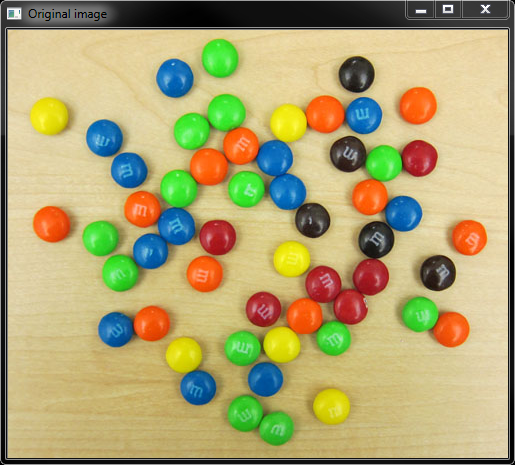
\includegraphics[width=0.45\textwidth]{Original_image.png}
	\caption{Načtený barevný obrázek ve vytvořeném okně.}	
\end{figure}
}






%-------------------------------------------------------------------------
\subsection{Načtení a vykreslení obrázku v odstínech šedi}

\par{Pro načtení obrázku v odstínech šedi je možné využít funkci \href{http://docs.opencv.org/modules/highgui/doc/reading_and_writing_images_and_video.html?highlight=imread#cv2.imread}{\textit{imread}} následovně
\lstinputlisting[firstline=66, lastline=67]{./code/MPV_cviceni_01_ucitel_p01.py}
nebo jej převést do požadovaného barevného prostoru pomocí funkce \href{http://docs.opencv.org/modules/imgproc/doc/miscellaneous_transformations.html?highlight=cvtcolor#cv2.cvtColor}{\textit{cvtColor}} následujícím způsobem
\lstinputlisting[firstline=44, lastline=45]{./code/MPV_cviceni_01_ucitel_p01.py}

\begin{figure}[!ht]
	\centering
	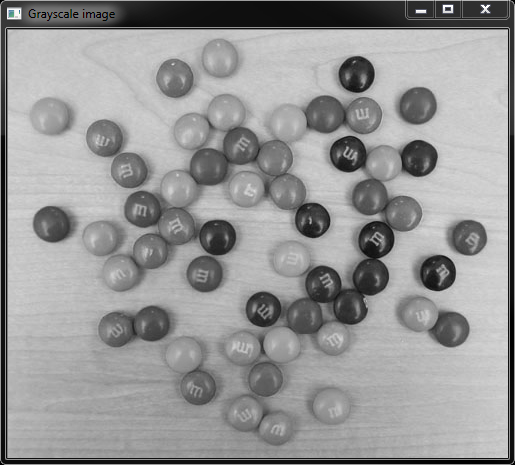
\includegraphics[width=0.45\textwidth]{GS_image.png}
	\caption{Načtený obrázek v odstínech šedi ve vytvořeném okně.}	
\end{figure}

}







\subsection{Výpočet histogramu a distribuční funkce}
\par{Pro výpočet histogramu se využije tento známý obrázek (je hojně využíván pro výpočet hloubkové mapy), který se načte
\lstinputlisting[firstline=67, lastline=67]{./code/MPV_cviceni_01_ucitel_p01.py}
\begin{figure}[!ht]
	\centering
	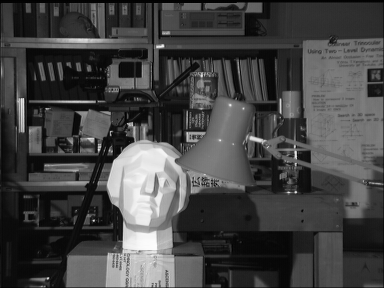
\includegraphics[width=0.45\textwidth]{tsukuba_r.png}
	\caption{Vstupní obrázek v odstínech šedi.}	
\end{figure}
Pro výpočet histogramu lze použít funkci \href{http://docs.scipy.org/doc/numpy/reference/generated/numpy.histogram.html}{\textit{histogram}} následovně,
\lstinputlisting[firstline=71, lastline=72]{./code/MPV_cviceni_01_ucitel_p01.py}
kde první vstupní parametr je obrázek v odstínech šedi, který je transformován do 1D pole pomocí funkce \href{http://docs.scipy.org/doc/numpy/reference/generated/numpy.ndarray.flatten.html}{\textit{flatten}}, druhý použitý vstupní parametr udává počet binů (neboli počet sloupců v histogramu, v případě obrázku v odstínech šedi tento parametr nabývá hodnoty 256) a poslední použitý vstupní parametr reprezentuje rozsah hodnot sloupců. Výstupními parametry jsou hodnoty histogramu a hranice binů.
}

\par{Pro výpočet distribuční funkce histogramu stačí hodnoty histogramu sečíst pomocí funkce \href{http://docs.scipy.org/doc/numpy/reference/generated/numpy.cumsum.html}{\textit{cumsum}}
\lstinputlisting[firstline=74, lastline=76]{./code/MPV_cviceni_01_ucitel_p01.py}
a znormovat pro vykreslení.
\lstinputlisting[firstline=78, lastline=79]{./code/MPV_cviceni_01_ucitel_p01.py}
}

\par{Nyní zbývá histogram společně s distribuční funkcí vykreslit. Vytvoření figury, do které se bude následně vykreslovat
\lstinputlisting[firstline=81, lastline=82]{./code/MPV_cviceni_01_ucitel_p01.py}
vykreslení distribuční funkce modrou barvou,
\lstinputlisting[firstline=84, lastline=85]{./code/MPV_cviceni_01_ucitel_p01.py}
~\\
vykreslení histogramu červenou barvou,
\lstinputlisting[firstline=87, lastline=88]{./code/MPV_cviceni_01_ucitel_p01.py}
nastavení limitů $x$-ové osy,
\lstinputlisting[firstline=90, lastline=91]{./code/MPV_cviceni_01_ucitel_p01.py}
vykreslení legendy
\lstinputlisting[firstline=93, lastline=95]{./code/MPV_cviceni_01_ucitel_p01.py}
a závěrečné vykreslení grafu.
\lstinputlisting[firstline=97, lastline=98]{./code/MPV_cviceni_01_ucitel_p01.py}

\begin{figure}[!ht]
	\centering
	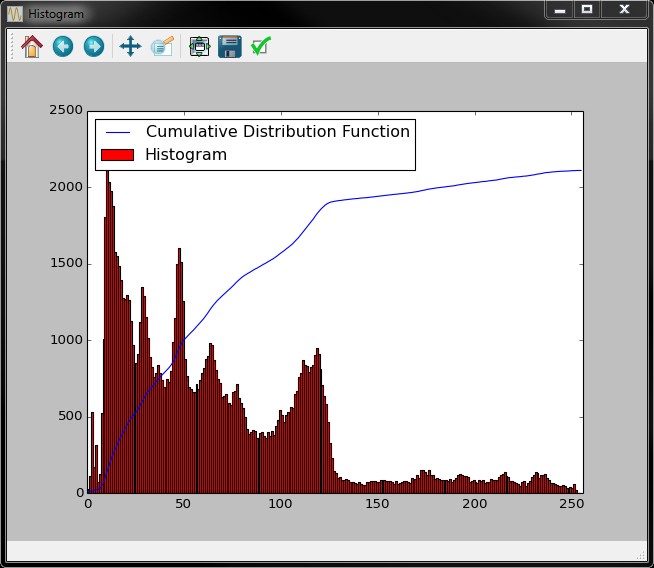
\includegraphics[width=0.5\textwidth]{GS_histogram.png}
	\caption{Histogram načteného obrázku v odstínech šedi.}	
\end{figure}

}






\newpage










%-------------------------------------------------------------------------
\subsection{Globální ekvalizace histogramu}

\par{Pro výpočet globální ekvalizace histogramu lze použít funkci \href{http://docs.opencv.org/modules/imgproc/doc/histograms.html?highlight=equalizehist#cv2.equalizeHist}{\textit{equalizeHist}}, která na vstup vyžaduje šedotónový obrázek.
\lstinputlisting[firstline=118, lastline=119]{./code/MPV_cviceni_01_ucitel_p01.py}
Výsledný ekvalizovaný histogram společně s distribuční funkcí lze vidět na Obr. \ref{fig:GSEQ_histogram} a porovnání originálního a ekvalizovaného obrázku lze vidět na Obr. \ref{fig:GSvsEQ_image}.
\begin{figure}[!ht]
	\centering
	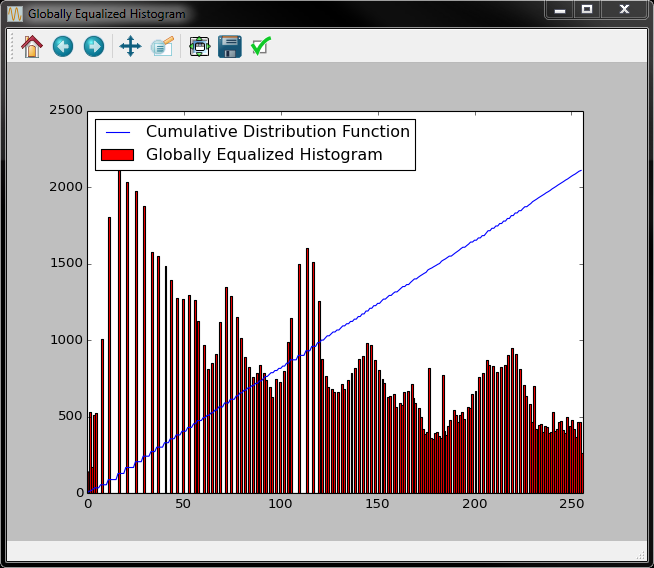
\includegraphics[width=0.5\textwidth]{GSEQ_histogram.png}
	\caption{Globálně ekvalizovaný histogram.}	
	\label{fig:GSEQ_histogram}
\end{figure}
\begin{figure}[!ht]
	\centering
	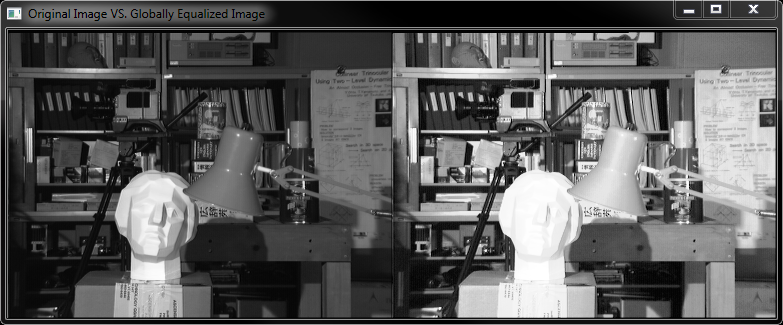
\includegraphics[width=1\textwidth]{GSvsEQ_image.png}
	\caption{Porovnání originálního a ekvalizovaného obrázku.}	
	\label{fig:GSvsEQ_image}
\end{figure}}










\newpage










%-------------------------------------------------------------------------
\subsection{Contrast Limited Adaptive Histogram Equalization}
\label{sec:CLAHE}

\par{Pro výpočet Contrast Limited Adaptive Histogram Equalization (CLAHE) je nutné nejprve vytvořit objekt pomocí funkce \textit{createCLAHE}
\lstinputlisting[firstline=171, lastline=172]{./code/MPV_cviceni_01_ucitel_p01.py}
dále se aplikuje na vstupní obrázek v odstínech šedi.
\lstinputlisting[firstline=174, lastline=175]{./code/MPV_cviceni_01_ucitel_p01.py}
Výsledný ekvalizovaný histogram pomocí metody CLAHE společně s~distribuční funkcí lze vidět na Obr. \ref{fig:GSEQCLAHE_histogram} a~porovnání originálního obrázku, globálně ekvalizovaného obrázku a~obrázku ekvalizovaného metodou CLAHE lze vidět na Obr. \ref{fig:GSvsEQvsCLAHE_image}.
\begin{figure}[!ht]
	\centering
	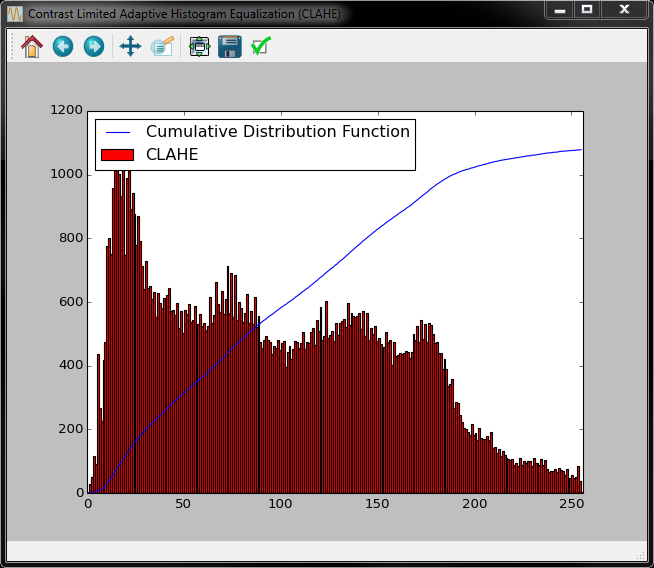
\includegraphics[width=0.5\textwidth]{GSEQCLAHE_histogram.png}
	\caption{Histogram metody CLAHE.}	
	\label{fig:GSEQCLAHE_histogram}
\end{figure}
\begin{figure}[!ht]
	\centering
	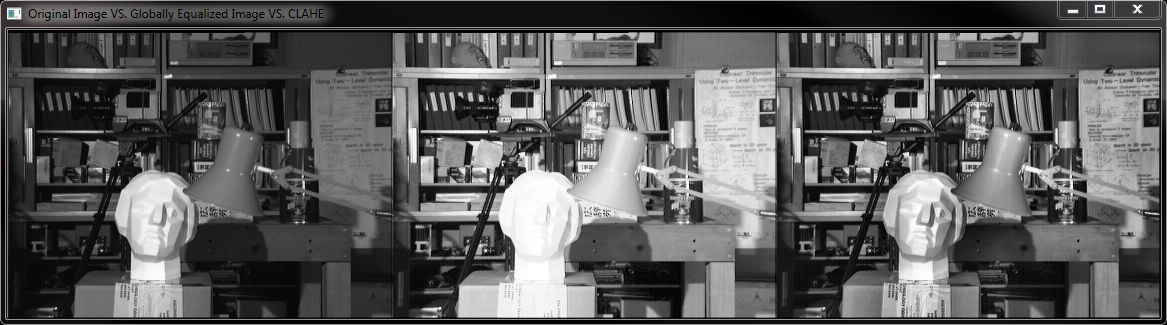
\includegraphics[width=1\textwidth]{GSvsEQvsCLAHE_image.png}
	\caption{Porovnání originálního obrázku, globálně ekvalizovaného obrázku a obrázku ekvalizovaného metodou CLAHE.} 	
	\label{fig:GSvsEQvsCLAHE_image}
\end{figure}}







\newpage











%-------------------------------------------------------------------------
\subsection{Otsuova metoda prahování}
\label{sec:Otsu}
\par{Pro ukázku \href{http://en.wikipedia.org/wiki/Otsu's_method}{Otsuovo metody prahování} bude použit následující obrázek obsahující scénu se zrnky rýže, na kterých je patrný gradientní přechod světla, proto obyčejné prahování nemá šanci uspokojivě oddělit popředí od pozadí.
\begin{figure}[!ht]
	\centering
	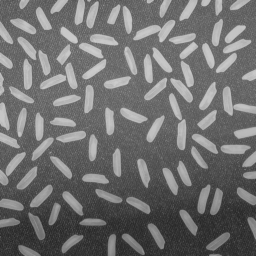
\includegraphics[width=0.45\textwidth]{rice.jpg}
	\caption{Obrázek zrnek rýže obsahující gradientní přechod světla.} 	
	\label{fig:rice}
\end{figure}
Na obrázek byla nejdříve aplikována metoda CLAHE (viz podsekce \ref{sec:CLAHE}) a následně Otsuova metoda pomocí funkce \href{http://docs.opencv.org/modules/imgproc/doc/miscellaneous_transformations.html?highlight=threshold#cv2.threshold}{\textit{threshold}}.
\lstinputlisting[firstline=257, lastline=259]{./code/MPV_cviceni_01_ucitel_p01.py}
Výsledek prahování lze vidět na Obr. \ref{fig:threshold_rice}.
\begin{figure}[!ht]
	\centering
	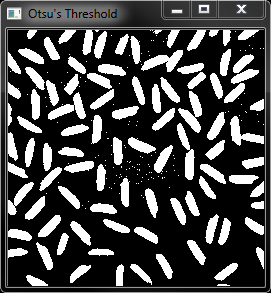
\includegraphics[width=0.45\textwidth]{threshold_rice.png}
	\caption{Výsledek prahování.}
	\label{fig:threshold_rice}
\end{figure}
}







\newpage








%-------------------------------------------------------------------------
\subsection{Počítání objektů}

\par{Počítání objektů je jedna z důležitých úloh počítačového vidění. Bude využit výsledek z~podkapitoly \ref{sec:Otsu} z~Obr. \ref{fig:threshold_rice}. Na tomto obrázku jsou patrné malé bílé objekty, které nereprezentují zrnka rýže, ale byly způsobeny šumem. Proto je dobré je odstranit, k~čemuž bude využito morfologické operace otevření se strukturním elementem $3 \times 3$ se počátkem uprostřed. Morfologickou operaci otevření provedeme pomocí OpenCV funkce \href{http://docs.opencv.org/modules/imgproc/doc/filtering.html?highlight=morphologyex#cv2.morphologyEx}{\textit{morphologyEx}}, která na vstup vyžaduje vstupní obrázek, jaká operace má být provedena s jakým strukturním elementem a kolik iterací dané operace se má provést. Funkce vrací výsledný obrázek.
\lstinputlisting[firstline=271, lastline=277]{./code/MPV_cviceni_01_ucitel_p01.py}
Pro určení počtu objektů ve scéně je možné využít funkce \href{http://docs.opencv.org/modules/imgproc/doc/structural_analysis_and_shape_descriptors.html?highlight=findcontours#cv2.findContours}{\textit{findContours}}, která nalezne obrysy objektů v binárním obraze.
\lstinputlisting[firstline=279, lastline=281]{./code/MPV_cviceni_01_ucitel_p01.py}
Na závěr je možné nalezené obrysy vykreslit pomocí funkce \href{http://docs.opencv.org/modules/imgproc/doc/structural_analysis_and_shape_descriptors.html?highlight=drawcontours#cv2.drawContours}{\textit{drawContours}}. Přičemž ucelenější kód lze nalézt níže.
\lstinputlisting[firstline=283, lastline=313]{./code/MPV_cviceni_01_ucitel_p01.py}
Výsledný počet obrysů objektů z Obr. \ref{fig:contours_rice} je roven 95, jak je možné vidět, tak některá zrnka jsou spojena do jednoho objektu, proto je zde prostor pro vylepšení.
\begin{figure}[!ht]
	\centering
	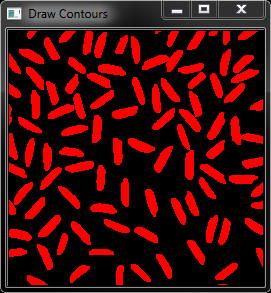
\includegraphics[width=0.45\textwidth]{contours_rice.png}
	\caption{Vykreslené obrysy objektů.}
	\label{fig:contours_rice}
\end{figure}
}

\newpage















%--------PRAKTICKE-CVICENI-CAST-2.---------------------------------------
\section{Praktické cvičení část 2.}

\subsection*{Non-maximum suppression}
\par{Non-maximum suppression je metoda pro nalezení maxim (potlačení nemaxim), která se využívá například při hledání maxim v histogramu a následném prahování více prahy.}

\begin{figure}[!ht]
	\centering
	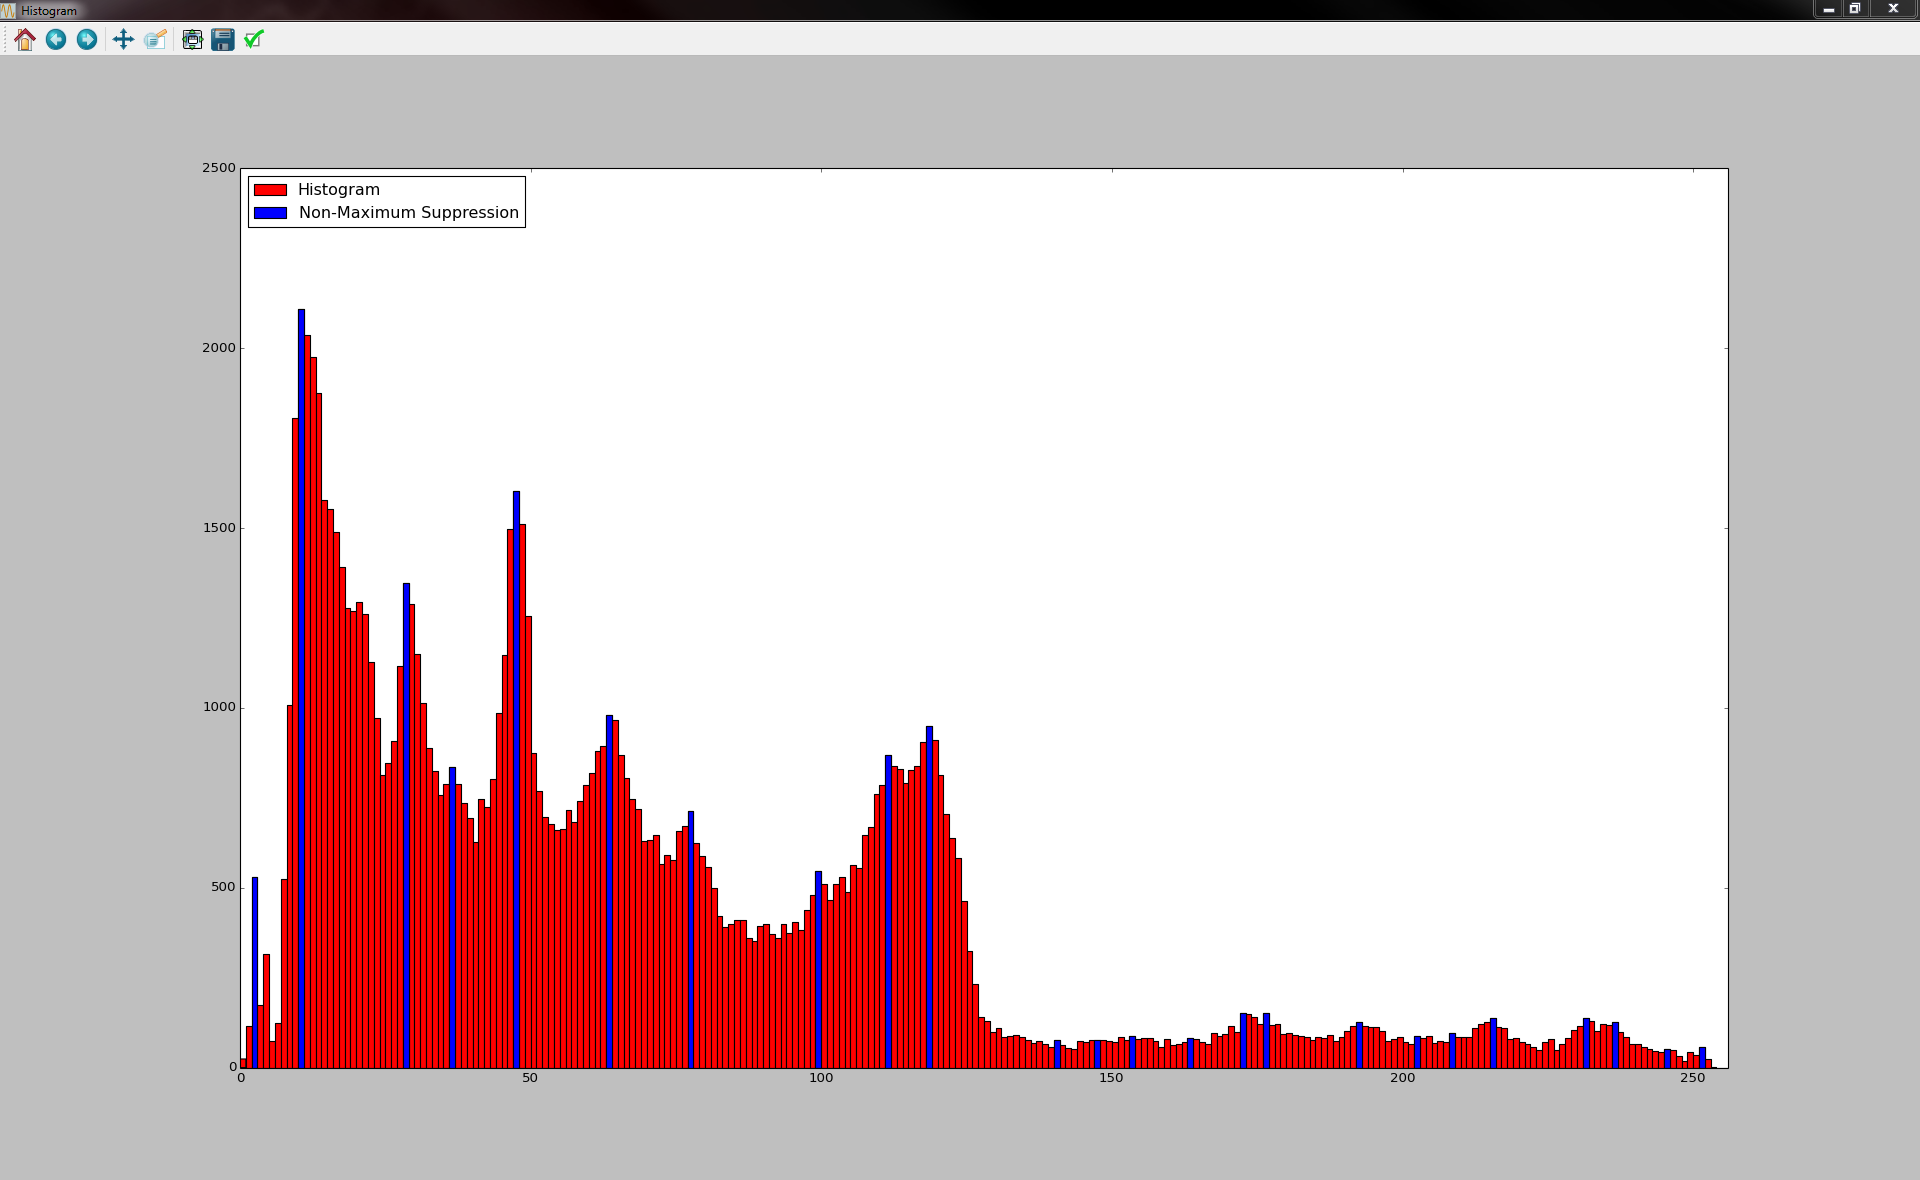
\includegraphics[width=0.8\textwidth]{Non_maximum_suppression.png}
	\caption{Histogram s vyznačenými nalezenými maximy s okénkem o velikosti 7.}
	\label{fig:Non_maximum_suppression}
\end{figure}

\begin{figure}[!ht]
	\centering
	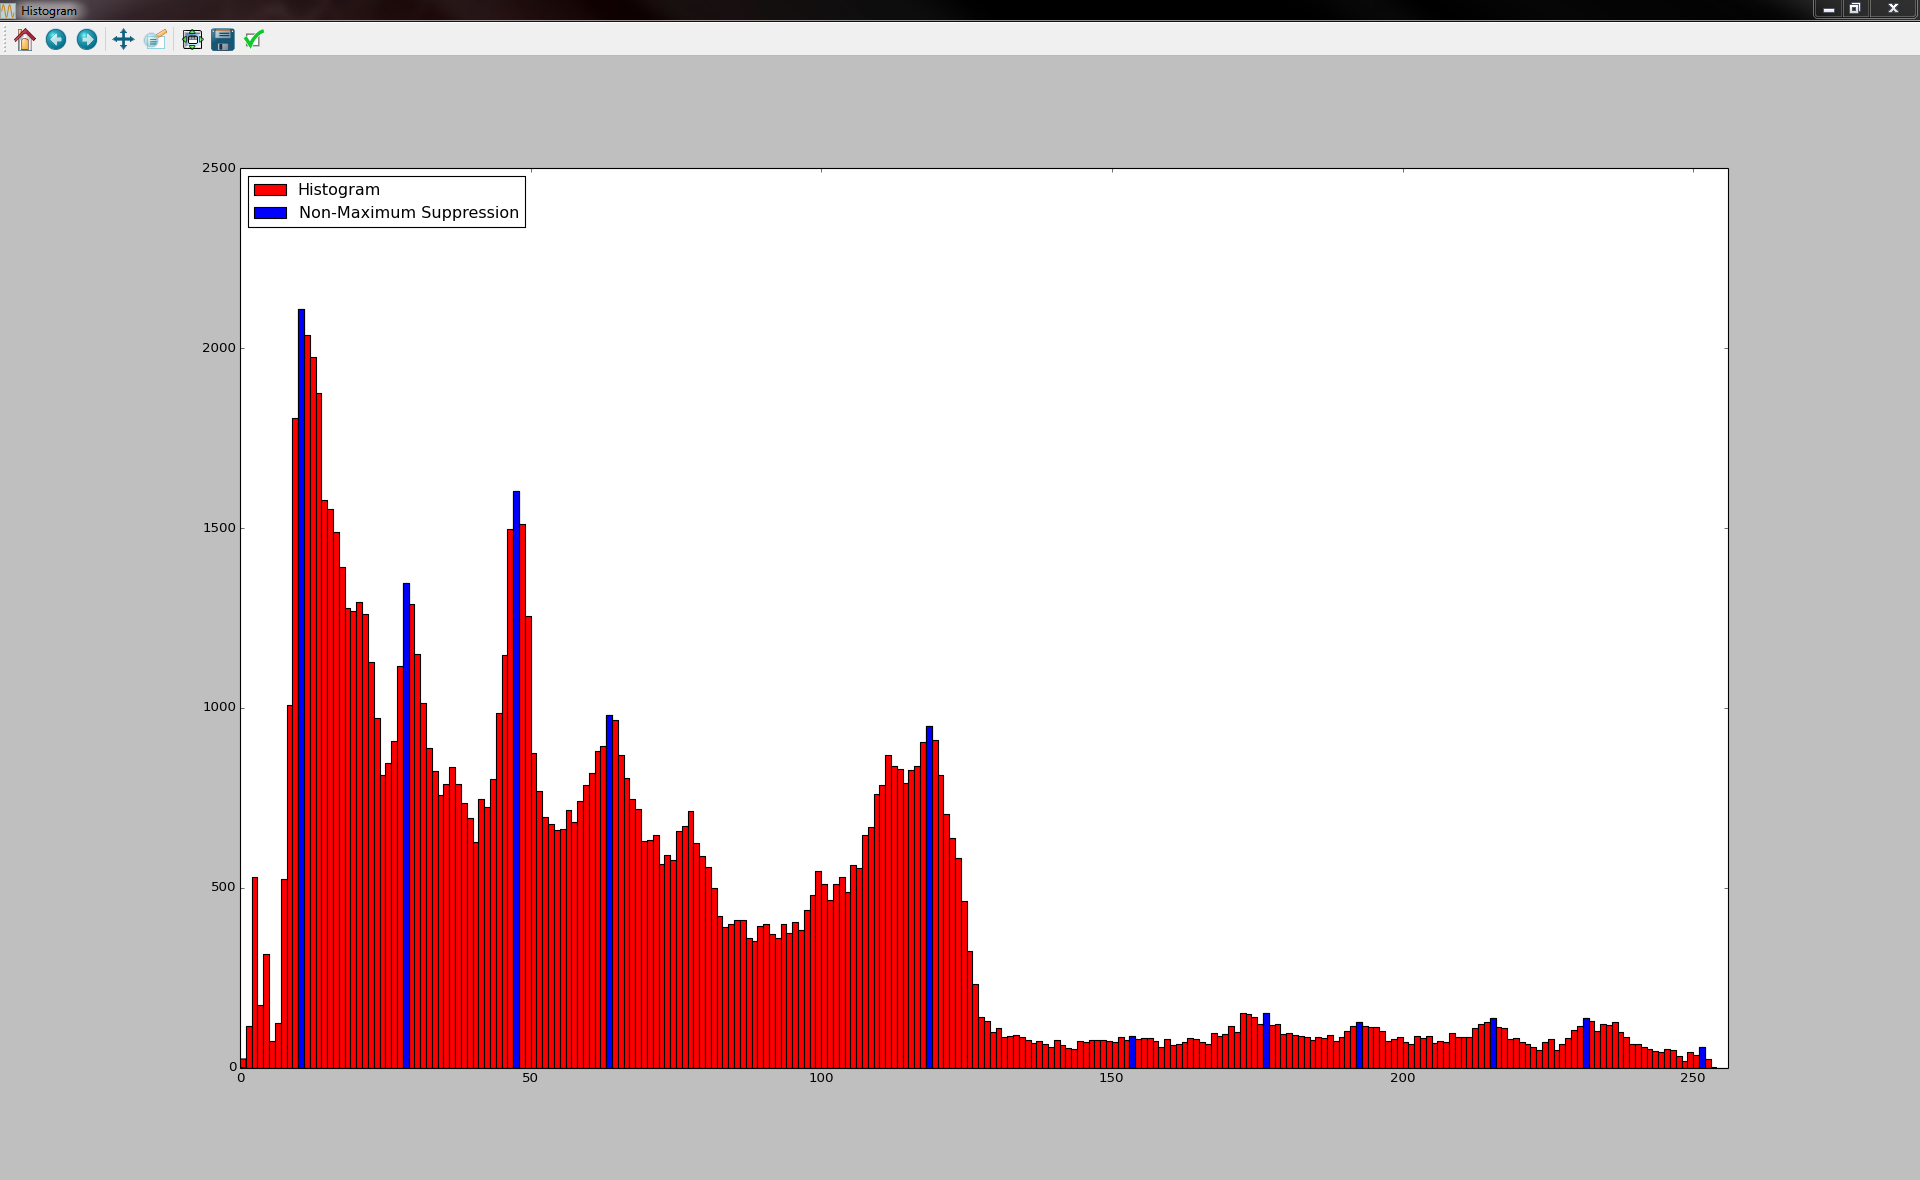
\includegraphics[width=0.8\textwidth]{Non_maximum_suppression02.png}
	\caption{Histogram s vyznačenými nalezenými maximy s okénkem o velikosti 21.}
	\label{fig:Non_maximum_suppression02}
\end{figure}

\newpage

\begin{figure}[!ht]
	\centering
	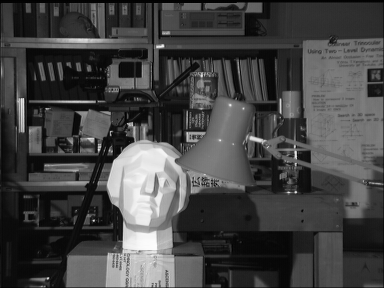
\includegraphics[width=0.45\textwidth]{tsukuba_r.png}
	\caption{Vstupní obrázek v odstínech šedi.}	
	\label{fig:input}
\end{figure}

\begin{figure}[!ht]
	\centering
	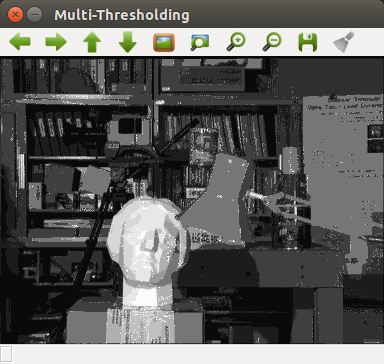
\includegraphics[width=0.45\textwidth]{Multi_thresholding.png}
	\caption{Vstupní obrázek prahovaný 11 prahy s hodnotami v obrázku získanými z pozic maxim v Obr. \ref{fig:Non_maximum_suppression02}.}
	\label{fig:Multi_thresholding}
\end{figure}








\end{document}



















